% ============================================================================
% v4 (fourth revision): reorganized per the Word draft, prior-projection track.
% Compile with pdflatex/tectonic: figures are PNGs in the same directory.
% ============================================================================
\ifdefined\XeTeXversion\else\pdfoutput=1\fi
\documentclass[10pt]{article}

\usepackage[margin=1in]{geometry}
\usepackage{amsmath,amssymb}
\usepackage{booktabs}
\usepackage{microtype}
\usepackage{graphicx}
\usepackage{xcolor}
\usepackage{enumitem}
\usepackage{needspace}
\usepackage[hidelinks]{hyperref}

\newcommand{\method}{APCS}
\newcommand{\kv}{KV}
\newcommand{\chg}{\text{CHG}}
\newcommand{\tgrr}{\text{TGRR}}
\newcommand{\psr}{\text{PSR}}
\newcommand{\pcr}{\text{PCR}}

\title{Beyond Cache Emulation: Advantage-Preserving Large-to-Small KV State Handoff without Re-Prefill}
\author{Anonymous Authors}
\date{}

\begin{document}
\maketitle

\begin{abstract}
Large language model systems increasingly rely on model routing, mid-session switching, and
multi-agent collaboration, yet a receiver typically has to prefill the full context again after a
model switch. Prior work separately establishes the feasibility of cross-model KV replacement and
semantic communication through latent/KV states, but leaves a stronger question open: can a weaker
student that never constructs context self-KV consume only a stronger teacher's runtime state and
inherit part of the teacher's task advantage? We study Advantage-Preserving Large-to-Small KV
Handoff and introduce \method, which separates state synthesis into a student-compatible base and
an advantage-carrying state. Before offline experiments, we use a conservative prior projection
(not measured evidence) to make the hypothesis quantitatively falsifiable, and we report it as
ranges rather than fabricated point estimates so that a pre-registered hypothesis is not mistaken
for a measured result. For Qwen3-4B$\rightarrow$1.7B at 4K, we project that a ridge replacement
retains roughly 92--96\% of the student self-prefill score while still showing \chg{} in the
$-2$ to $-4$ pp band; a low-rank compatibility base retains roughly 90--94\% at $\pcr\approx0.23$;
and full \method{} plausibly lands in a \chg{} range of about $-1.5$ to $+3$ pp
(\tgrr{} roughly $-15\%$ to $+30\%$), a range whose central tendency is only mildly positive and
does not exclude zero, while retaining on the order of 8--16\% student-side prefill saving.
A single-GPU cost projection suggests little or negative benefit at very short contexts, with the
map/load-versus-prefill break-even plausibly falling somewhere in the 4K--8K range rather than at a
single fixed point, since part of the mapping cost may itself scale with context length. These
values are experimental priors only, deliberately left wide to reflect genuine pre-experiment
uncertainty; every quantitative claim in the submission will be replaced by frozen-test, multi-seed,
measured P50/P95 results.
\end{abstract}

\section{Introduction}
When one model finishes reading a long context and a second, smaller model takes over, the second
model normally has to re-read the whole context. Prefill is already the dominant cost of
long-context inference, and multi-model serving makes that cost recur: routing, mid-session
switching, and multi-agent setups pass the same context between models, and each receiver pays the
prefill again.

Existing systems reuse a cache only within one model, or they impose architectural constraints.
DroidSpeak shares KV state across fine-tuned variants of one architecture, ICaRus and PrefillShare
redesign the model so several decoders share a prefill module, and Cross-Model KV Cache Transfer
learns closed-form ridge or MLP mappings that let a receiver skip prefill for matched-KV pairs
inside one family. A second line of work treats states as a communication medium: Cache-to-Cache
fuses source KV into the receiver's own state, LatentAlign aligns KV latent spaces, and Latent
Cache Flow compresses cache-level communication. None of these asks whether the receiver can do
better than its own full-prefill baseline.

We ask that question directly: does part of the task advantage of a stronger teacher live in the
runtime KV state, in a form a weaker student can consume without re-reading the original context
and without changing the student's weights? A positive answer would turn cross-model KV handoff
from redundant-compute elimination into runtime capability transfer. A negative answer would draw
a clean boundary between state compatibility and capability transfer. Both outcomes are useful,
which is why the paper is organized around a falsifiable probe rather than a promised gain.

The paper makes three contributions: a problem definition (advantage-preserving large-to-small KV
handoff, with \chg{} and \psr{} as the joint criterion), a method that separates a
student-compatible base state from an advantage-carrying state (\method), and an experimental
characterization plan that treats teacher gap, model-size gap, context length, and mapper budget
as variables and reports direction asymmetry rather than hiding it.

\begin{figure}[t]
\centering
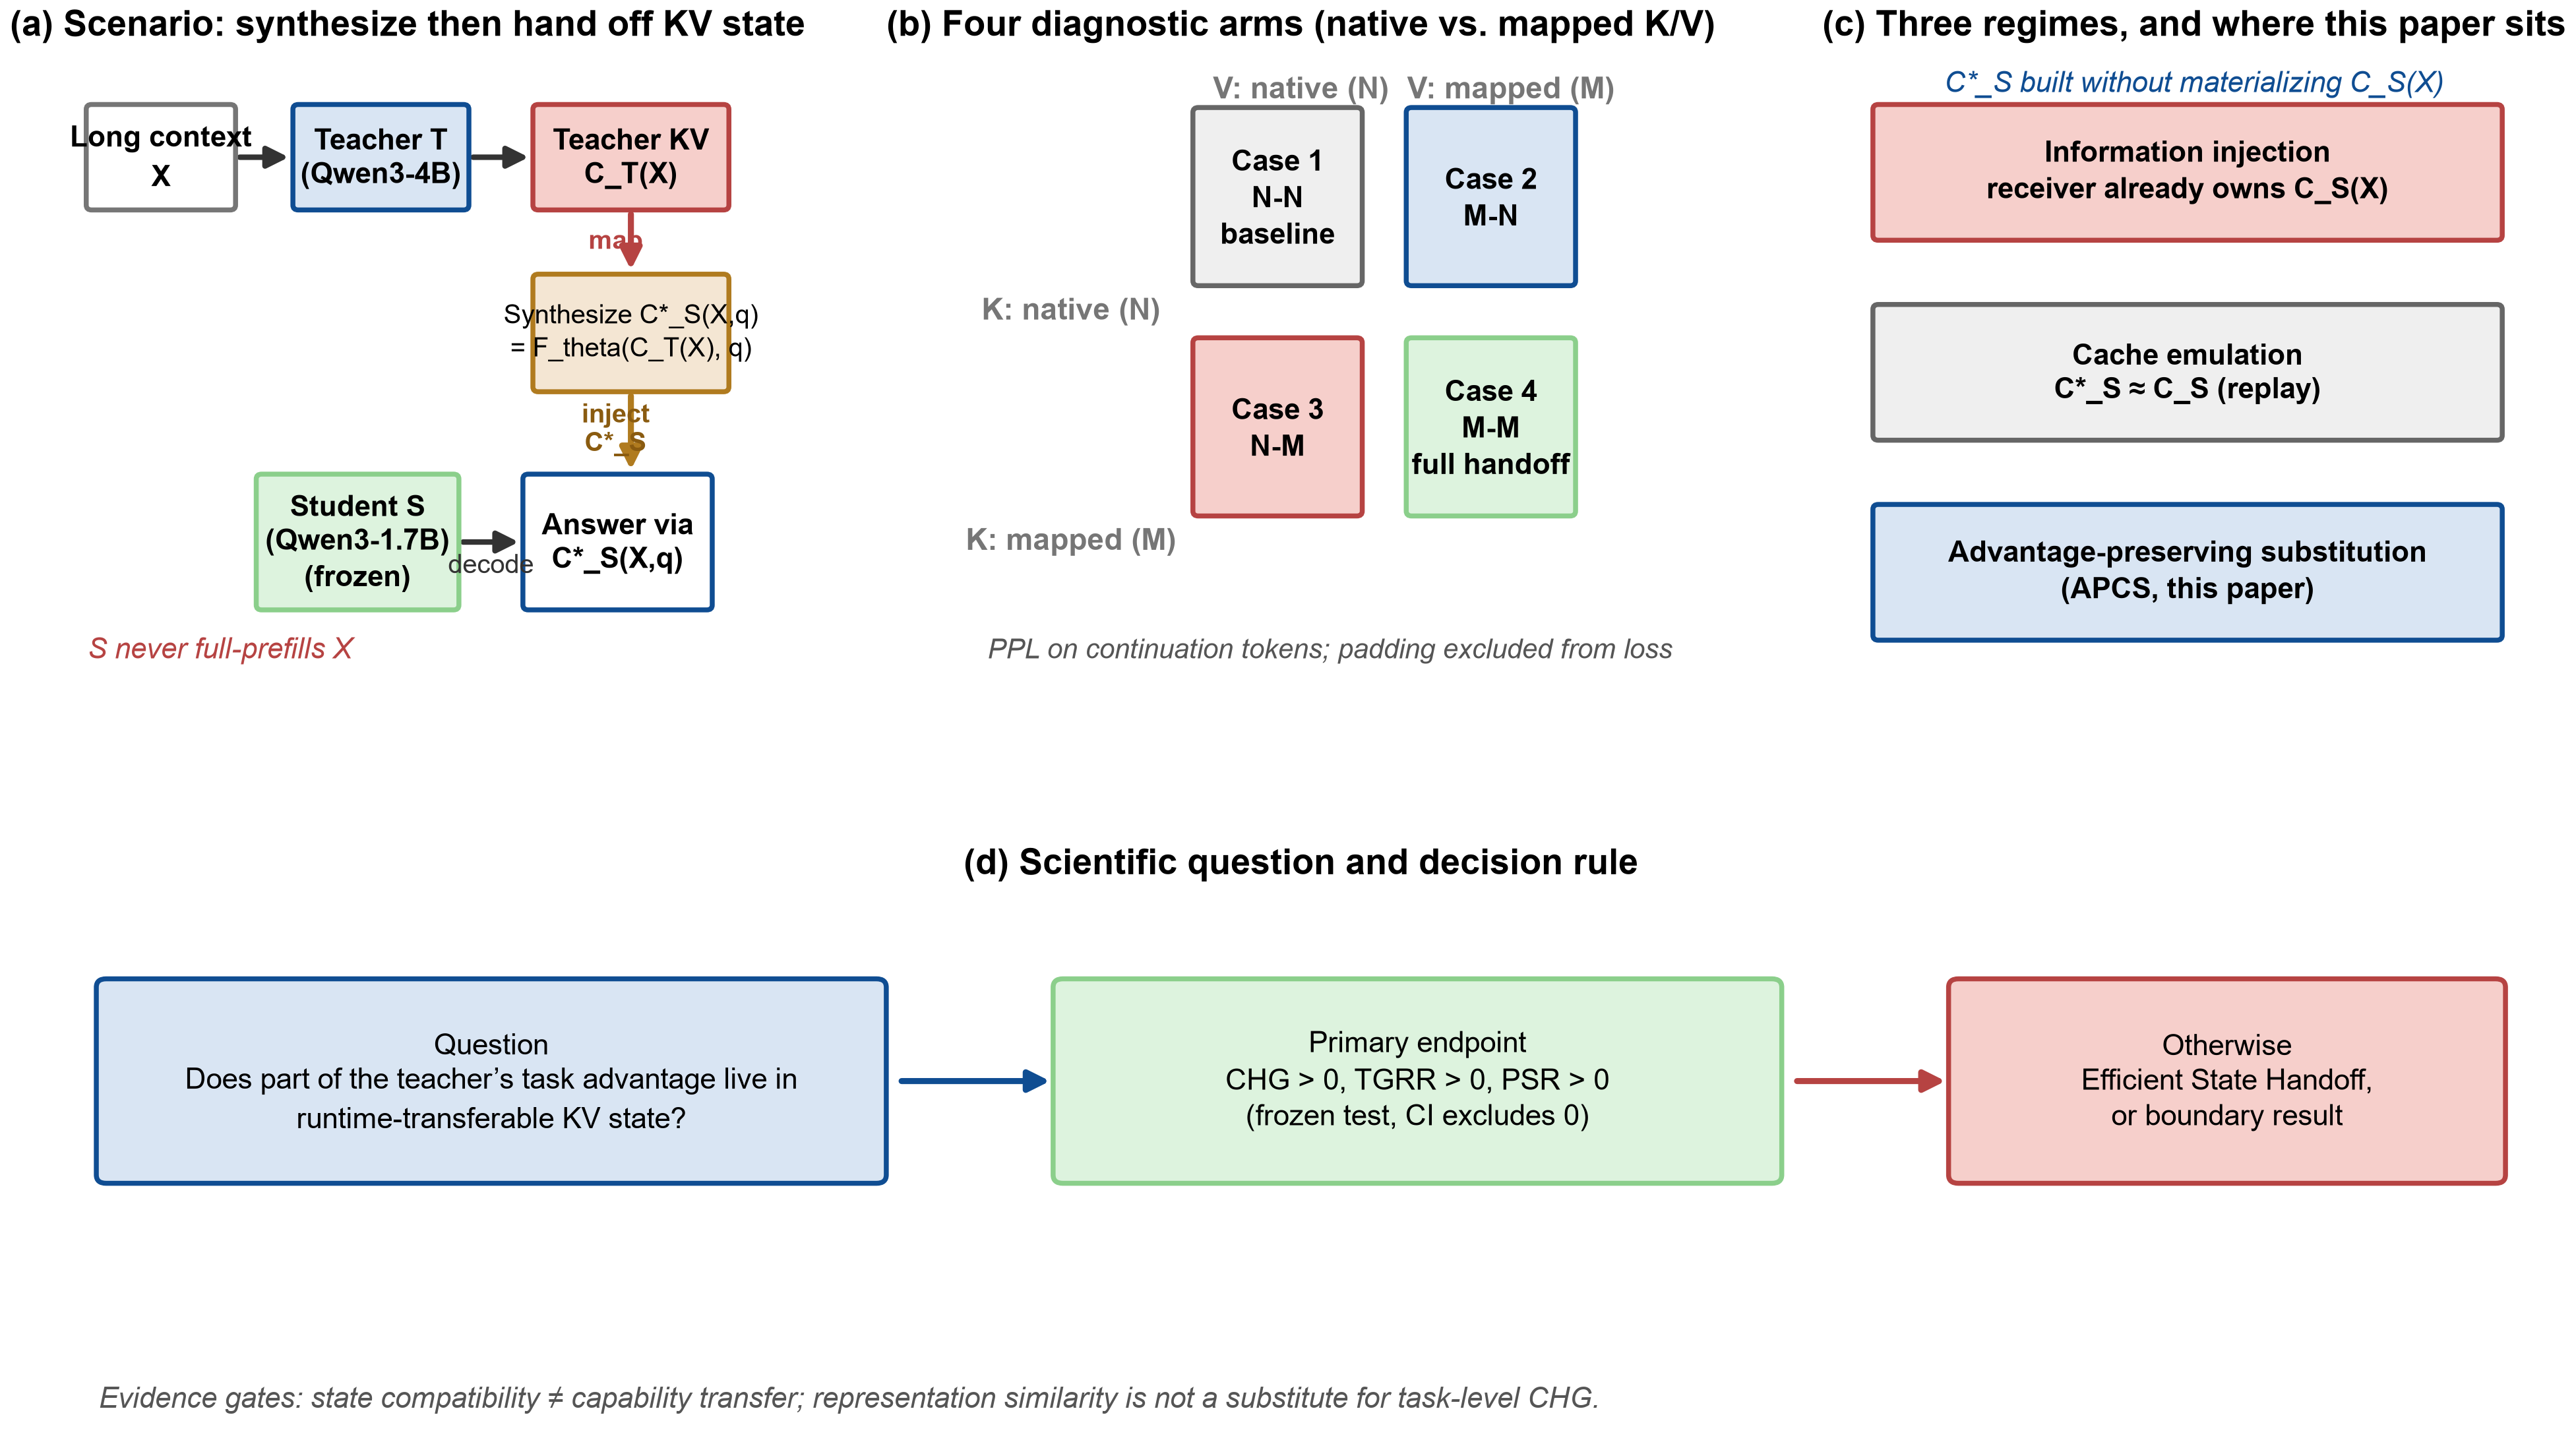
\includegraphics[width=0.96\textwidth]{figure1_problem_analysis.png}
\caption{Problem setup and research question. (a) The teacher reads a long context and produces KV
state; a mapper synthesizes a student-compatible cache $C_S^*(X,q)=F_\theta(C_T(X),q)$, which is
injected into the frozen student without full prefill. (b) The four diagnostic arms switch native
and mapped K/V. (c) How this setting differs from information injection and cache emulation.
(d) The decision rule: capability transfer if \chg{}, \tgrr{}, and \psr{} are positive on frozen
tests, otherwise Efficient State Handoff or a boundary result.}
\label{fig:problem}
\end{figure}

\section{Related Work}
\subsection{KV Cache and the Economics of Prefill}
A Transformer prefill pass processes all input tokens in parallel and stores layer-wise keys and
values for subsequent autoregressive decoding. FlashAttention and FlashAttention-2 substantially
improve attention IO efficiency, but they do not remove redundant prefill when a second model must
reprocess the same long context \cite{dao2022flashattention,dao2024flashattention2}.
PagedAttention/vLLM reduces KV fragmentation and enables intra-model cache sharing, while Mooncake
and LMCache elevate KV state into a transferable storage object across GPU, CPU, SSD, and
inference engines \cite{kwon2023vllm,qin2025mooncake,cheng2025lmcache}. These systems motivate our
cost accounting but predominantly assume state reuse within the same model.

\subsection{Cross-Model KV Reuse and Prefill Replacement}
DroidSpeak targets fine-tuned model variants with the same architecture and selectively recomputes
a small set of critical layers while reusing the remaining KV state. ICaRus conceptually
factorizes a decoder-only Transformer into a logical encoder that produces KV states and a logical
decoder that predicts tokens, enabling multiple specialized decoders to share an identical cache.
PrefillShare similarly introduces a shared prefill module with specialized decoding modules. These
works establish cross-model redundant prefill as a systems problem, but they impose architectural
or training-time constraints.

The closest replacement baseline is Cross-Model KV Cache Transfer \cite{heo2026crossmodel}. For
within-family pairs with matched KV-head count and per-head dimension, it selects top-$k$
predictive source layers, removes RoPE from keys before fitting, and learns per-head ridge mappings
from source to receiver KV. Its results directly establish the feasibility of receiver-free
cross-size state replacement, so neither receiver-free inference nor a linear mapper is a novelty
claim of this work. Our optimization target is different: rather than projecting teacher state
back toward the student's self-prefill state as faithfully as possible, we ask whether a
receiver-consumable state can preserve useful teacher-only task advantage.

\subsection{KV/Latent States as an Inter-Model Communication Medium}
C2C trains a neural projector that fuses a source model's KV cache into the target model's own KV
cache and gates the layers that benefit from communication \cite{fu2025c2c}. LatentAlign maps
multiple models into and out of a shared KV latent space \cite{dery2026latentalign}. LCF compresses
cache-level communication and transmits information absent from the receiver context
\cite{rossi2026latentcacheflow}. KaVa further shows that compressed teacher KV trajectories can
act as supervision for latent-reasoning students \cite{kuzina2026kava}. These works support the
premise that runtime states contain semantically useful signals, but they do not answer our strict
substitution setting because the receiver typically has its own context-derived state or the
transfer occurs during training rather than runtime handoff.

\subsection{Behavioral Stability and Long-Context Evaluation}
Numerical KV similarity alone is an incomplete fidelity criterion. Heo et al.\ report that
attention-output cosine is more predictive of downstream retention than raw KV $R^2$
\cite{heo2026crossmodel}. Liang et al.\ show an even stronger failure mode: KV reuse can preserve
end-task accuracy while substantially changing an LLM judge's candidate-selection behavior,
motivating Judge Consistency Rate and cross-candidate attention diagnostics
\cite{liang2026kvjudge}. We therefore evaluate representation-, attention-, behavior-, and
task-level fidelity. For long contexts, LongBench, RULER, and LongBench Pro provide complementary
realistic and controllable evaluation regimes \cite{bai2023longbench,hsieh2024ruler,chen2026longbenchpro}.

\section{Problem Formulation}
\subsection{Setting}
Let $X$ denote a long context, $T$ a teacher model, $S$ a student model, and $q$ a later query.
The teacher has already processed $X$ as part of an upstream reading, reasoning, or conversational
stage and materialized its runtime KV state $C_T(X)$. The student is not allowed to full-prefill
$X$ and instead consumes a synthesized student-compatible cache:
\begin{equation}
  C_S^*(X,q) = F_\theta(C_T(X), q),
\label{eq:synthesis}
\end{equation}
\begin{equation}
  \hat y = S(q\,;\, C_S^*(X,q)), \qquad \mathrm{Prefill}_S(X) = 0.
\label{eq:no-prefill}
\end{equation}

\subsection{State Substitution versus Information Injection}
We distinguish three regimes. Information injection assumes that the receiver already owns
$C_S(X)$ and augments it with teacher information. Cache emulation constructs a state from
$C_T(X)$ that approximates the behavior of $C_S(X)$. Our target, advantage-preserving state
substitution, constructs $C_S^*$ without ever materializing $C_S(X)$ and asks whether this
substituted state can outperform the student self-prefill baseline. This distinction defines our
boundary with C2C/LCF and with conventional cross-model cache emulation.

\subsection{Metrics and Pareto Criterion}
\begin{align}
  \chg &= \mathrm{Score}_{\mathrm{handoff}} - \mathrm{Score}_{\mathrm{student\text{-}self}}, \\
  \tgrr &= \frac{\mathrm{Score}_{\mathrm{handoff}} - \mathrm{Score}_{\mathrm{student}}}
                 {\mathrm{Score}_{\mathrm{teacher}} - \mathrm{Score}_{\mathrm{student}}}, \\
  \psr &= 1 - \frac{T_{\mathrm{map}} + T_{\mathrm{load}} + T_{\mathrm{query}}}
                 {T_{\mathrm{prefill},S}(X)}, \\
  \pcr &= \frac{\mathrm{MapperSize}_{\mathrm{ours}}}{\mathrm{MapperSize}_{\mathrm{ridge}}}.
\end{align}
\chg{} is the primary scientific endpoint: it asks whether the handoff student exceeds its own
self-prefill baseline. \tgrr{} measures the fraction of the original teacher--student performance
gap recovered by handoff. \psr{} measures student-side prefill saving only in the main scenario
where the teacher cache already exists for an upstream reason. \pcr{} constrains deployment
footprint relative to the cross-model ridge mapper. We call $\chg>0$ together with $\psr>0$ a
Pareto Capability Handoff.

\section{Method: Advantage-Preserving Cache Synthesis}
\subsection{Design Principle}
\method{} starts from a tension between compatibility and advantage preservation. A mapper trained
only to minimize numerical error to the student self-KV may become very good at reproducing what
the student would have computed itself, while actively discarding teacher-specific state
directions that could improve the downstream task. We therefore separate two objectives: first
construct a stable receiver-consumable compatibility state; then learn a lightweight advantage
state that is not fully constrained to collapse back into the student self-prefill manifold.

\begin{figure}[t]
\centering
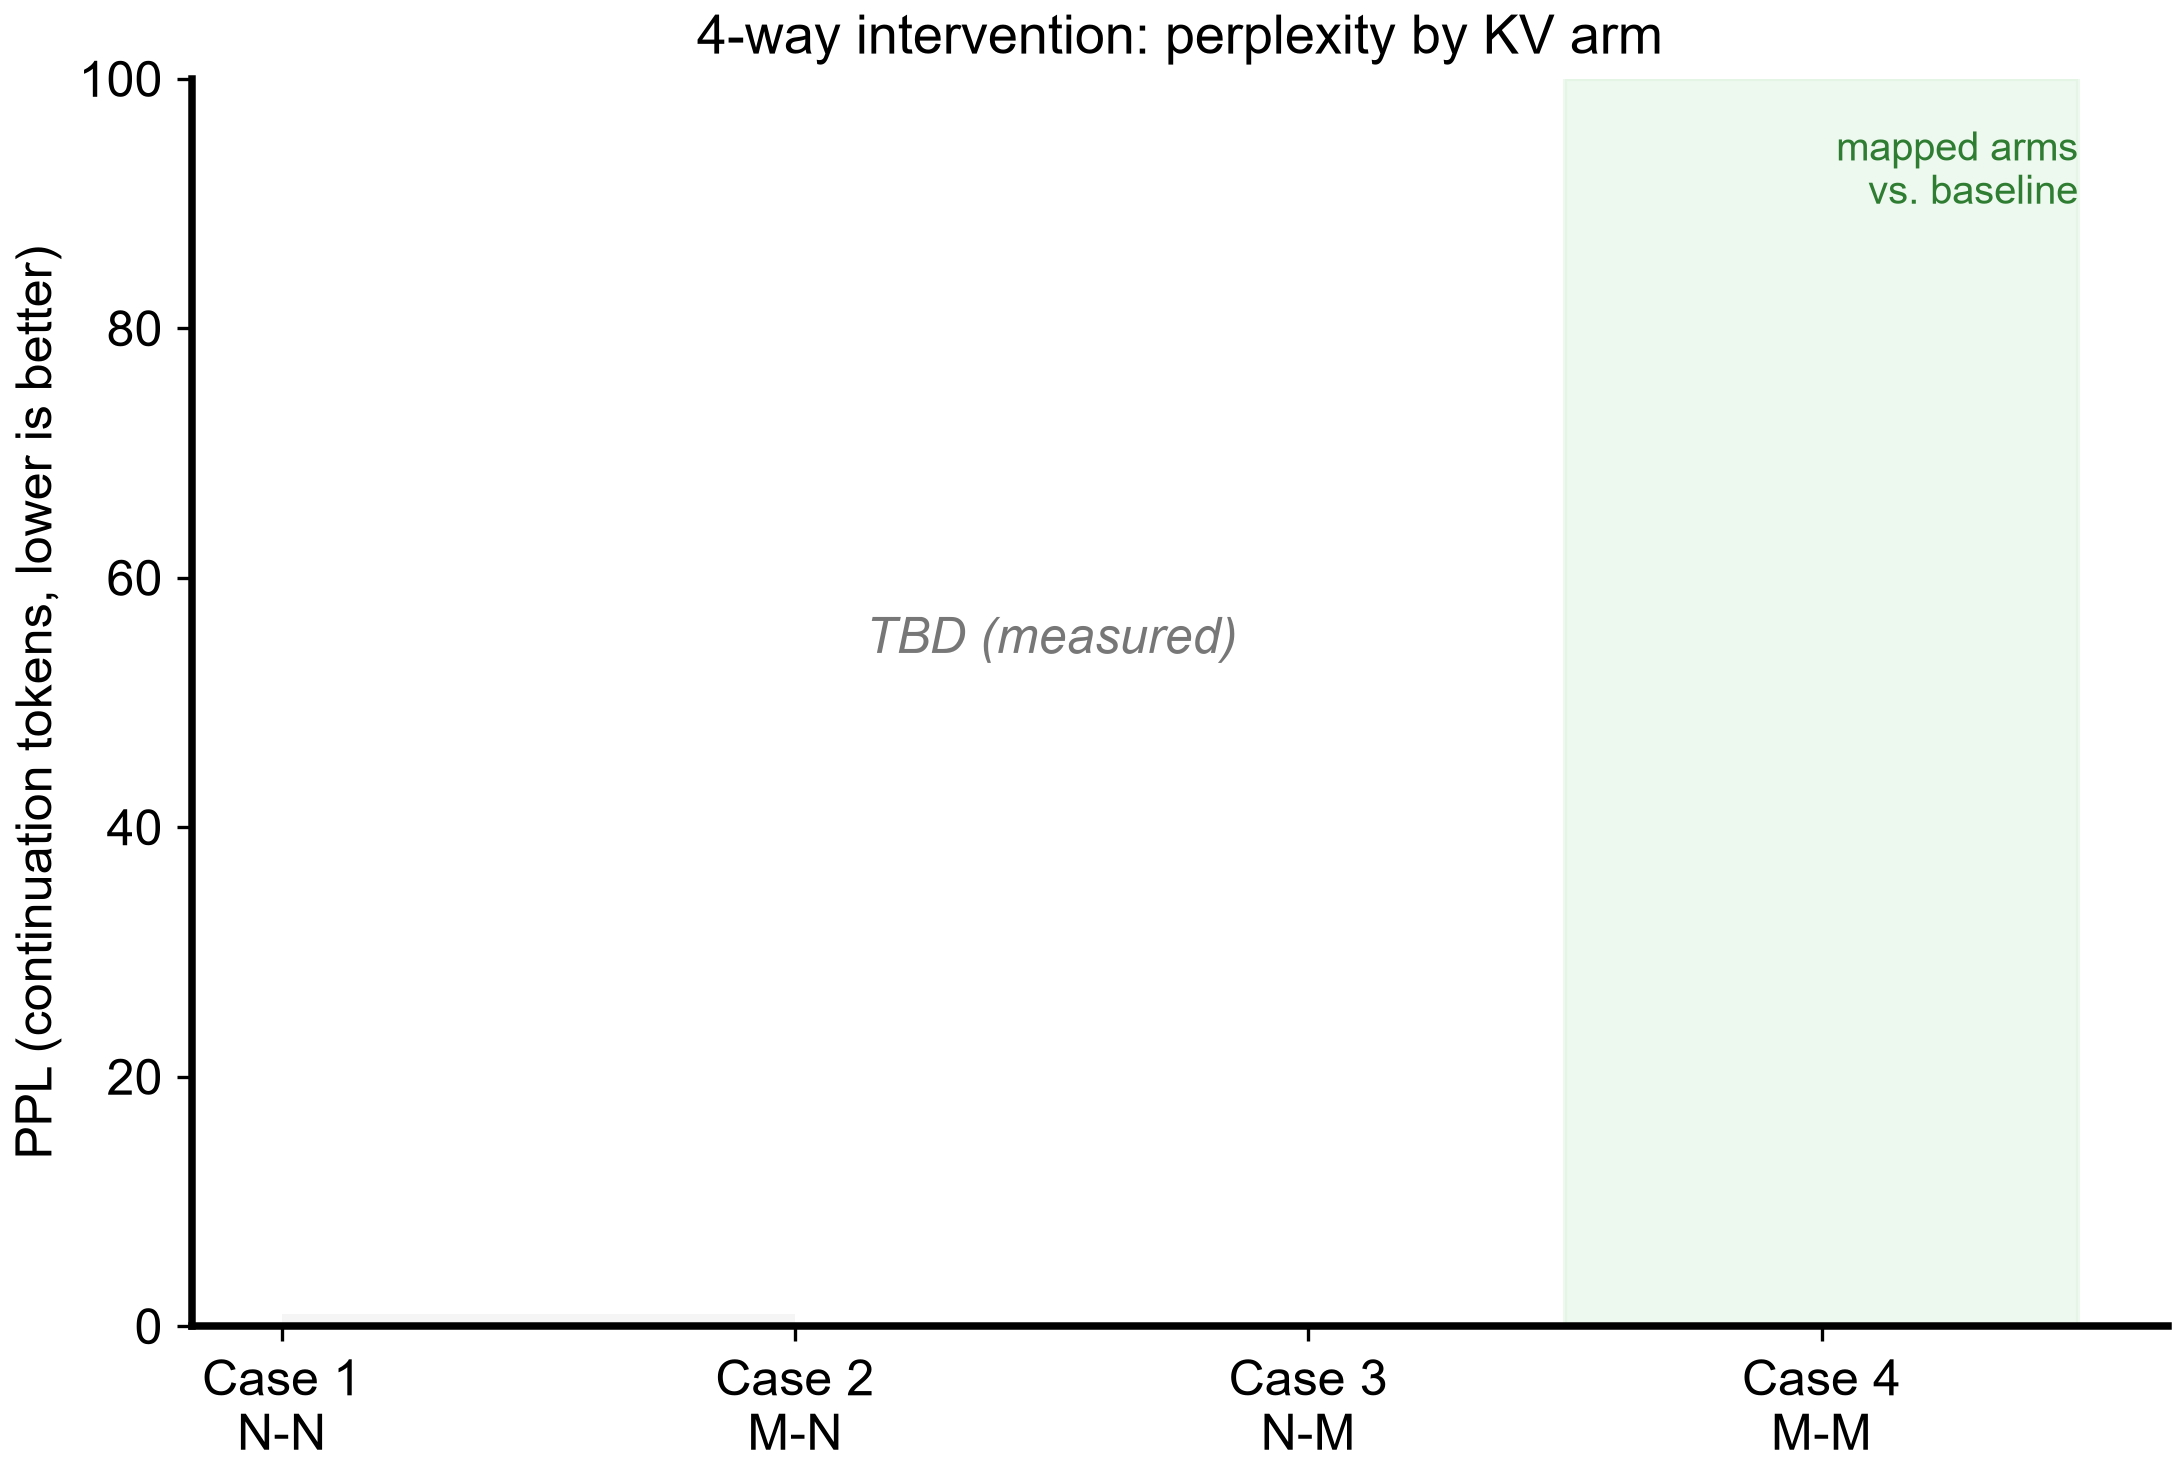
\includegraphics[width=0.62\textwidth]{figure2_fourway_ppl.png}
\caption{The four-way intervention design. Each arm is a different assignment of native or
ridge-mapped K and V to the student's \texttt{past\_key\_values}. PPL is computed on continuation
tokens with padding excluded from the loss; the mapped arms are highlighted because their gap to
the native baseline is the quantity of interest.}
\label{fig:fourway}
\end{figure}

\subsection{Compatibility Base}
\begin{equation}
  C_{\mathrm{base}}(X) = F_{\mathrm{compat}}(C_T(X)).
\label{eq:compat}
\end{equation}
$F_{\mathrm{compat}}$ begins from the strongest directly comparable replacement baseline. For each
student layer/head, we select top-$k$ teacher source layers; keys are mapped in de-RoPE content
space and then re-encoded with the student positional scheme; K and V are mapped separately. The
minimal-resource study first reproduces ridge regression and then explores low-rank factorization,
shared bases, and head/layer parameter sharing to reduce \pcr{} while maintaining retention.

\subsection{Advantage State}
\begin{equation}
  R_{\mathrm{adv}}(X) = E_{\mathrm{adv}}(C_T(X)).
\label{eq:adv}
\end{equation}
Once the compatibility base is stable, \method{} adds a lightweight advantage state $R_{\mathrm{adv}}$.
Unlike the base mapper, this branch is not forced to reconstruct the student self-KV; it is
supervised to retain teacher-conditioned directions that improve the downstream task while
remaining consumable by the frozen student. The minimal configuration uses a global or layer-wise
scalar $\alpha$:
\begin{equation}
  C_S^*(X) = C_{\mathrm{base}}(X) + \alpha \cdot R_{\mathrm{adv}}(X).
\label{eq:combine}
\end{equation}
A full configuration may later introduce lightweight query adaptation $g(q)$, but it must not
rescan the long teacher cache for each new query. All $O(|X|)$ context synthesis should happen
once; per-query adaptation should operate only over short-query features and layer/head or small
latent-slot gates.

\subsection{Training Objective}
\begin{equation}
  \mathcal{L}_{\method} = \mathcal{L}_{\mathrm{task}} + \lambda \mathcal{L}_{\mathrm{self}} +
  \lambda \mathcal{L}_{\mathrm{teacher}} + \lambda \mathcal{L}_{\mathrm{att}} +
  \lambda \mathcal{L}_{\mathrm{reg}}.
\label{eq:loss}
\end{equation}
$\mathcal{L}_{\mathrm{task}}$ directly optimizes the task answer or suffix generation objective.
$\mathcal{L}_{\mathrm{self}}$ stabilizes student behavior on examples where the teacher has little
advantage or may be wrong. $\mathcal{L}_{\mathrm{teacher}}$ provides teacher guidance only when a
teacher advantage is established on the training split. $\mathcal{L}_{\mathrm{att}}$ aligns
downstream-relevant attention outputs rather than only raw KV values. $\mathcal{L}_{\mathrm{reg}}$
controls rank, sparsity, or mapper budget. Teacher-advantage weights are computed exclusively from
training data; validation selects thresholds and hyperparameters; the test split remains frozen.

\subsection{Complexity and Deployment Accounting}
Our primary deployment scenario assumes the teacher cache already exists because the teacher
processed $X$ upstream, so the student-side handoff cost is map + cache load + query-only prefill.
If the teacher is invoked solely to create a transferable cache, teacher prefill must be included
and the reuse break-even must be reported.

\section{Experimental Setup}
\subsection{Research Phases and Models}
We begin with a minimal-resource probe: Qwen3-4B as teacher, Qwen3-1.7B as student, one NVIDIA GPU.
Qwen3-4B needs roughly 8GB in FP16/BF16 and Qwen3-1.7B roughly 3.5GB. With the sequential pipeline
of Section~5.5 (load the teacher, extract and save its KV cache, unload it, then load the
student), peak GPU memory stays below 12GB. The pair stays inside one family, which keeps
tokenizer, KV-head count, head dimension (128), and RoPE base compatible while preserving a real
size gap: 36 layers versus 28 \cite{yang2025qwen3}.

\subsection{Tasks and Data Splits}
The Fidelity Set measures whether handoff preserves basic student behavior and may include
HellaSwag, ARC-Challenge, selected MMLU tasks, and WinoGrande. The Teacher-Advantage Set is
selected only at the dataset level when the teacher reliably exceeds the student; individual test
examples are never filtered by teacher-win/student-loss outcomes. Long-context evaluation uses
LongBench/RULER-style tasks, starting at 4K before moving to 8K/16K/32K. A behavior-sensitive set
contains judge/ranker or multi-candidate comparison tasks to reveal decision drift that is not
visible in aggregate accuracy.

\subsection{Baselines}
\begin{itemize}[leftmargin=*,nosep]
  \item B0 Student Full Prefill: quality, behavior, and latency reference.
  \item B1 Teacher Full Inference: performance upper reference and teacher-gap definition.
  \item B2 Teacher Text/Summary Handoff $\rightarrow$ Student: conventional text-mediated communication.
  \item B3 Cross-Model Ridge Mapper: strongest directly comparable replacement baseline.
  \item B4 Cross-Model MLP: nonlinear repair baseline for difficult pairs.
  \item B5 C2C-style Fusion: capability-enhancement reference with a different receiver-state assumption.
  \item B6 LatentAlign / LCF: shared-latent and lightweight cache-communication references when code/checkpoints permit a fair comparison.
  \item O1 \method{} Base Only; O2 Base + Advantage State; O3 full \method{} if lightweight query adaptation is enabled.
\end{itemize}

\subsection{Metrics and Statistical Protocol}
All learned mappers/adapters use at least three random seeds. \chg{} confidence intervals and
significance are estimated with paired bootstrap or paired permutation tests whenever applicable.
Latency is measured after warm-up with repeated synchronized runs and reported at P50/P95,
separately accounting for mapping, CPU-to-GPU cache load, query-only prefill, decode, and student
full-prefill baseline. Every run fixes model commit, tokenizer, attention implementation, dtype,
RoPE configuration, cache layout, hardware, batch size, and context length.

\subsection{Minimal-Resource Implementation}
The study uses Hugging Face Transformers and controls \texttt{past\_key\_values} directly. One GPU
run follows this order: load teacher, forward and capture, move the needed state to CPU, unload
teacher, load student, map and inject, decode and evaluate. The two models are never resident at
the same time, so the peak stays below 12GB. Compute is small: the ridge fit uses head dimension
128 and the closed-form solution $(X^\top X + \lambda I)^{-1}X^\top Y$, so 100 calibration
examples of length 2048 fit in seconds; the 100-sample forward pass on the student takes minutes;
and the whole stage, debugging included, stays under half a day. Calibration uses 100 examples at
2048 tokens. The reference implementation and the three engineering details that keep the probe
valid are in Appendix~A.

\section{Expected Outcomes and Testable Predictions}
This section fixes expectations before the offline experiments and prevents post-hoc target
shifting. The numbers below are prior projections, not measurements, and must not be used as
submission claims. The projection assumes: ridge replacement mostly restores student behavior
rather than capability; any transferable teacher advantage is modest, on the order of 1--3
percentage points in this first small pair; and on a single GPU with sequential residency, map and
load overhead hurts short contexts and is amortized only as context grows.

\subsection{Reporting Convention: Ranges Instead of Fabricated Precision}
An earlier draft reported prior projections as single-decimal point estimates with seed-style
error bars and smooth curves, borrowing the visual grammar of measured multi-seed results for
numbers that were never measured. That presentation risks being read as evidence, so every prior
projection below is a range with an explicit central tendency, allowed to straddle zero when the
underlying hypothesis is genuinely uncertain. Every figure in this section shows a band, not a
line.

\begin{table}[t]
\centering
\caption{Prior-projected main results (NOT measured), reported as plausible ranges rather than
point estimates with fabricated seed variance. Values assume Qwen3-4B$\rightarrow$1.7B, 4K
context, and a frozen student. Student/Teacher are illustrative common composite task scores on a
0--100 scale.}
\label{tab:projection}
\small
\begin{tabular}{llrrrrrrrr}
\toprule
Method & Ctx & Student & Teacher & Handoff & Retention & CHG & TGRR & PSR & PCR \\
\midrule
Student Full Prefill & 4K & 54.8 & 64.7 & -- & 100.0\% & 0.0 & 0.0\% & 0.0\% & -- \\
Cross-Model Ridge & 4K & 54.8 & 64.7 & 50.4--52.6 & 92--96\% & $-4.4$ to $-2.2$ & $-44$ to $-22\%$ & 3--8\% & 1.00 \\
Low-rank Base & 4K & 54.8 & 64.7 & 49.3--51.5 & 90--94\% & $-5.5$ to $-3.3$ & $-56$ to $-33\%$ & 12--20\% & 0.23 \\
\method & 4K & 54.8 & 64.7 & 53.2--57.5 & 97--105\% & $-1.6$ to $+2.7$ & $-16$ to $+27\%$ & 8--16\% & 0.27 \\
\bottomrule
\end{tabular}
\end{table}

\subsection{Replacement Fidelity}
The prior projection deliberately separates replacement from capability transfer. Full ridge is
expected to reach roughly 92--96\% retention while still underperforming student self-prefill;
compressing the mapper to $\pcr\approx0.23$ is expected to lower retention only modestly, to
roughly 90--94\%. These bands, not single numbers, are the actual prediction: the published
cross-model ridge results that motivate them report a range of pair-dependent fidelities, and
there is no principled basis for asserting a single decimal before any Qwen3-4B$\rightarrow$1.7B
run has happened. If the measured curve falls inside this band, high-fidelity replacement and
positive capability transfer should still be treated as distinct gates rather than inferring
capability from KV or attention similarity.

\begin{figure}[t]
\centering
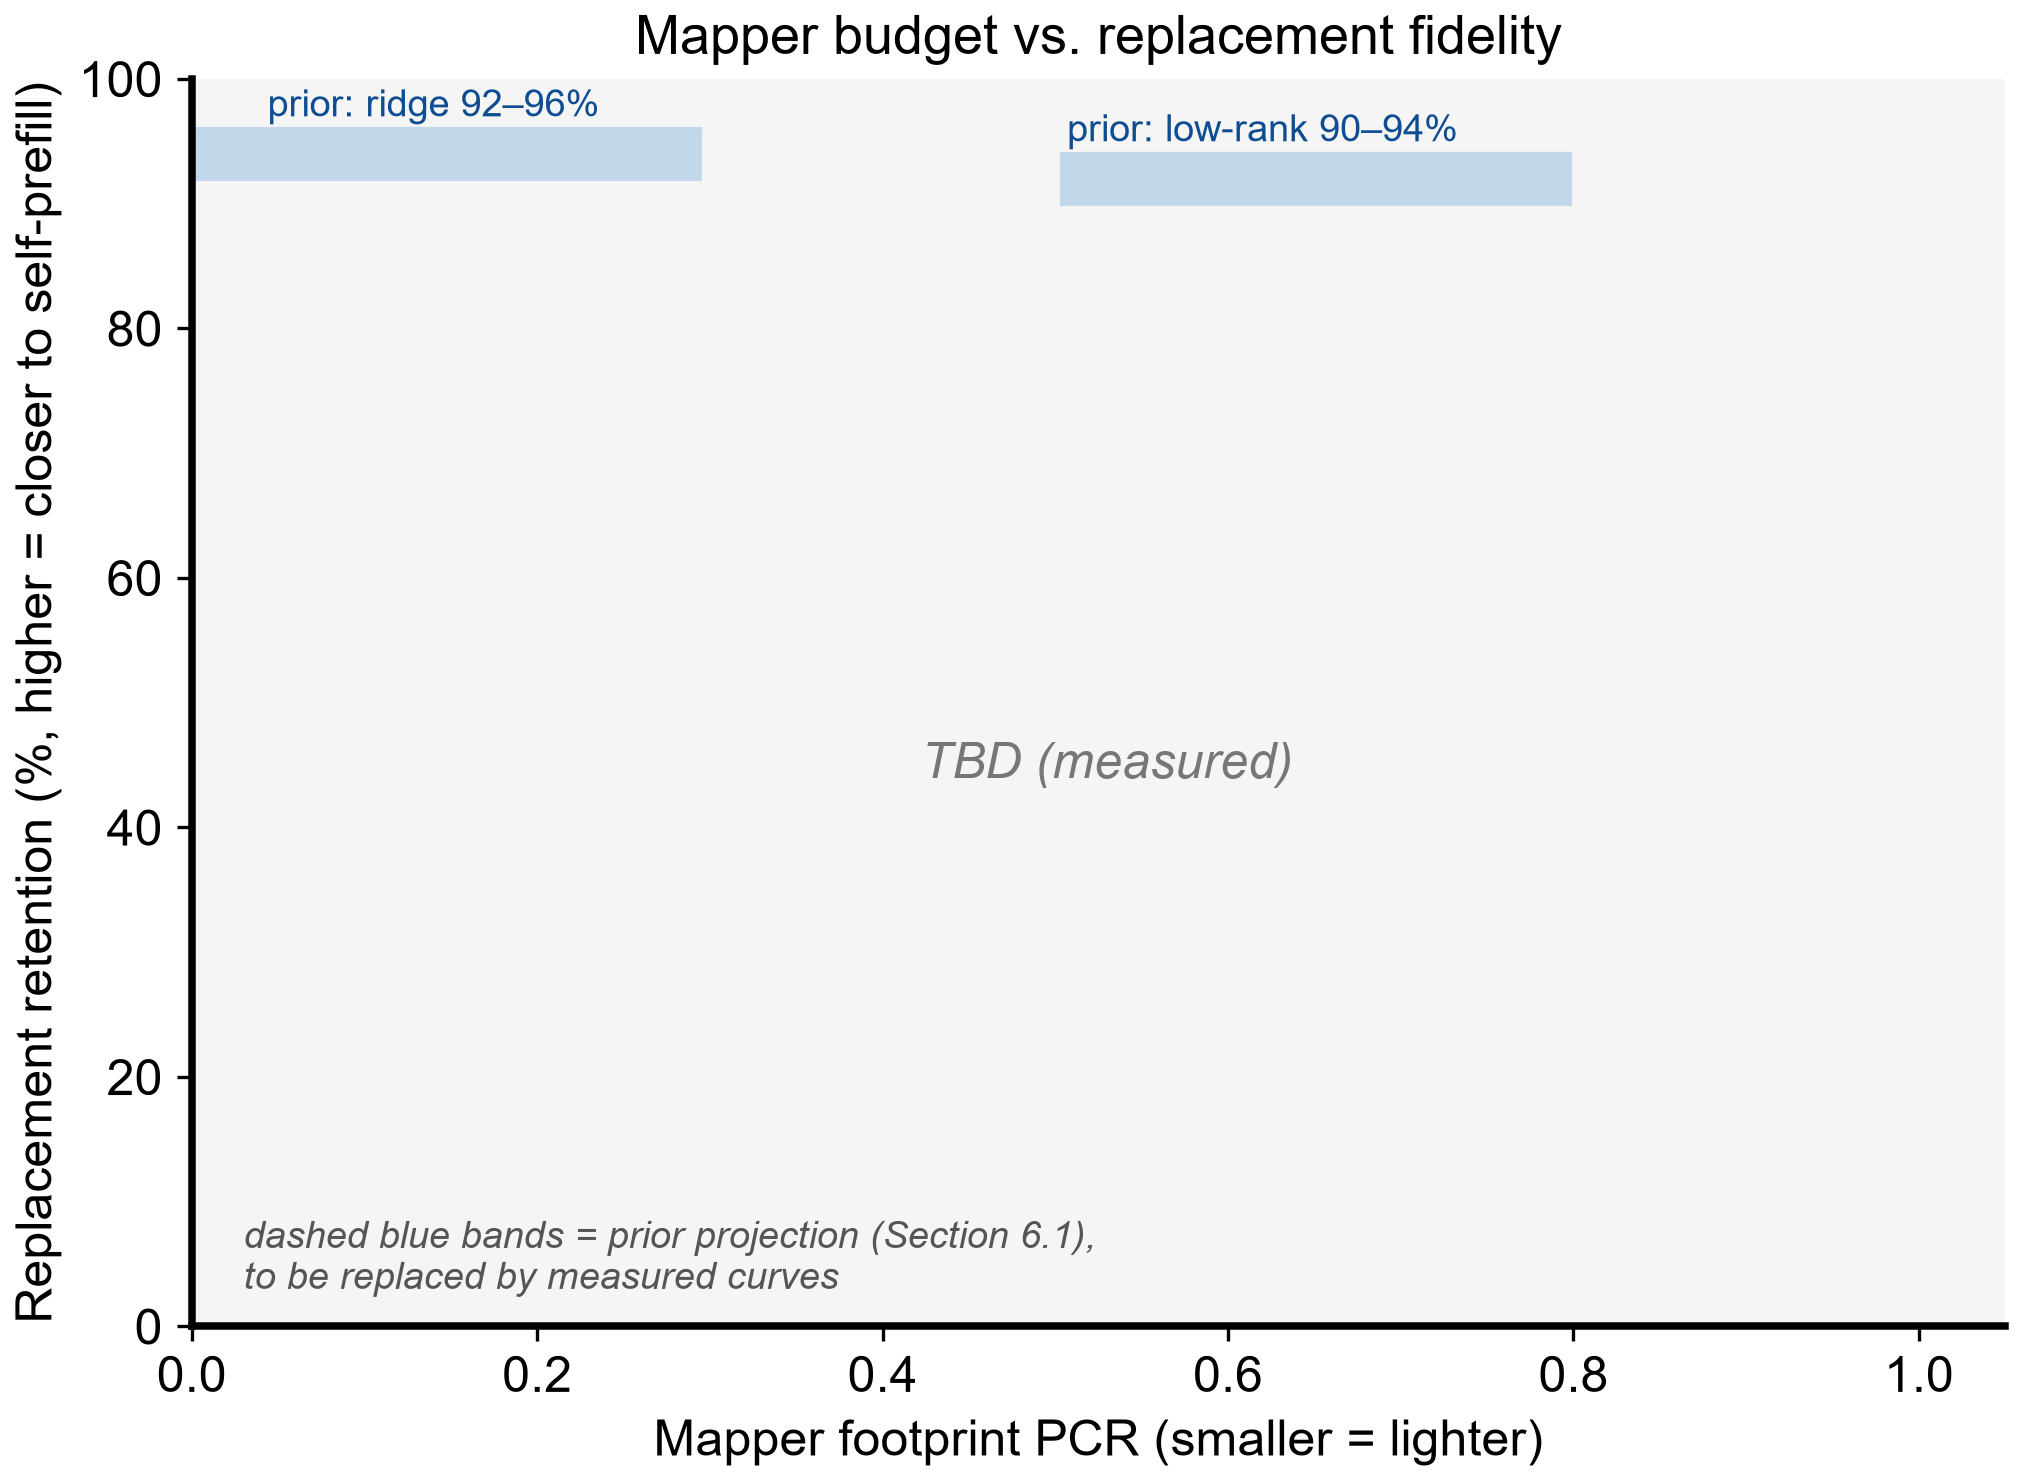
\includegraphics[width=0.60\textwidth]{figure3_pcr_retention.png}
\caption{Mapper footprint (\pcr) versus replacement retention. Dashed blue bands are prior
projections from Section~6.1; the measured curve is pending.}
\label{fig:pcr}
\end{figure}

\subsection{Teacher Advantage Transfer}
Under a wide but centered prior, full \method{} plausibly yields a full-test \chg{} somewhere in
the range of about $-1.6$ to $+2.7$ pp, corresponding to roughly $-16\%$ to $+27\%$ teacher-gap
recovery, a band whose midpoint is only mildly positive and does not rule out $\chg\le0$. More
importantly, the gain is projected to be heterogeneous with teacher gap: the plausible range for
\chg{} should include zero when the teacher gap is small (below roughly 3--5 pp), and only shift
confidently positive once the teacher exceeds the student by more than about 10 pp, with \tgrr{}
plausibly saturating somewhere between 10\% and 25\%. If observed, a widening gap between the
\chg{} range and zero as teacher gap grows would be stronger evidence for runtime-transferable
advantage than any single average accuracy delta; a flat, gap-independent \chg{} close to zero
would instead support the direction-asymmetry concern raised in Section~7.

\begin{figure}[t]
\centering
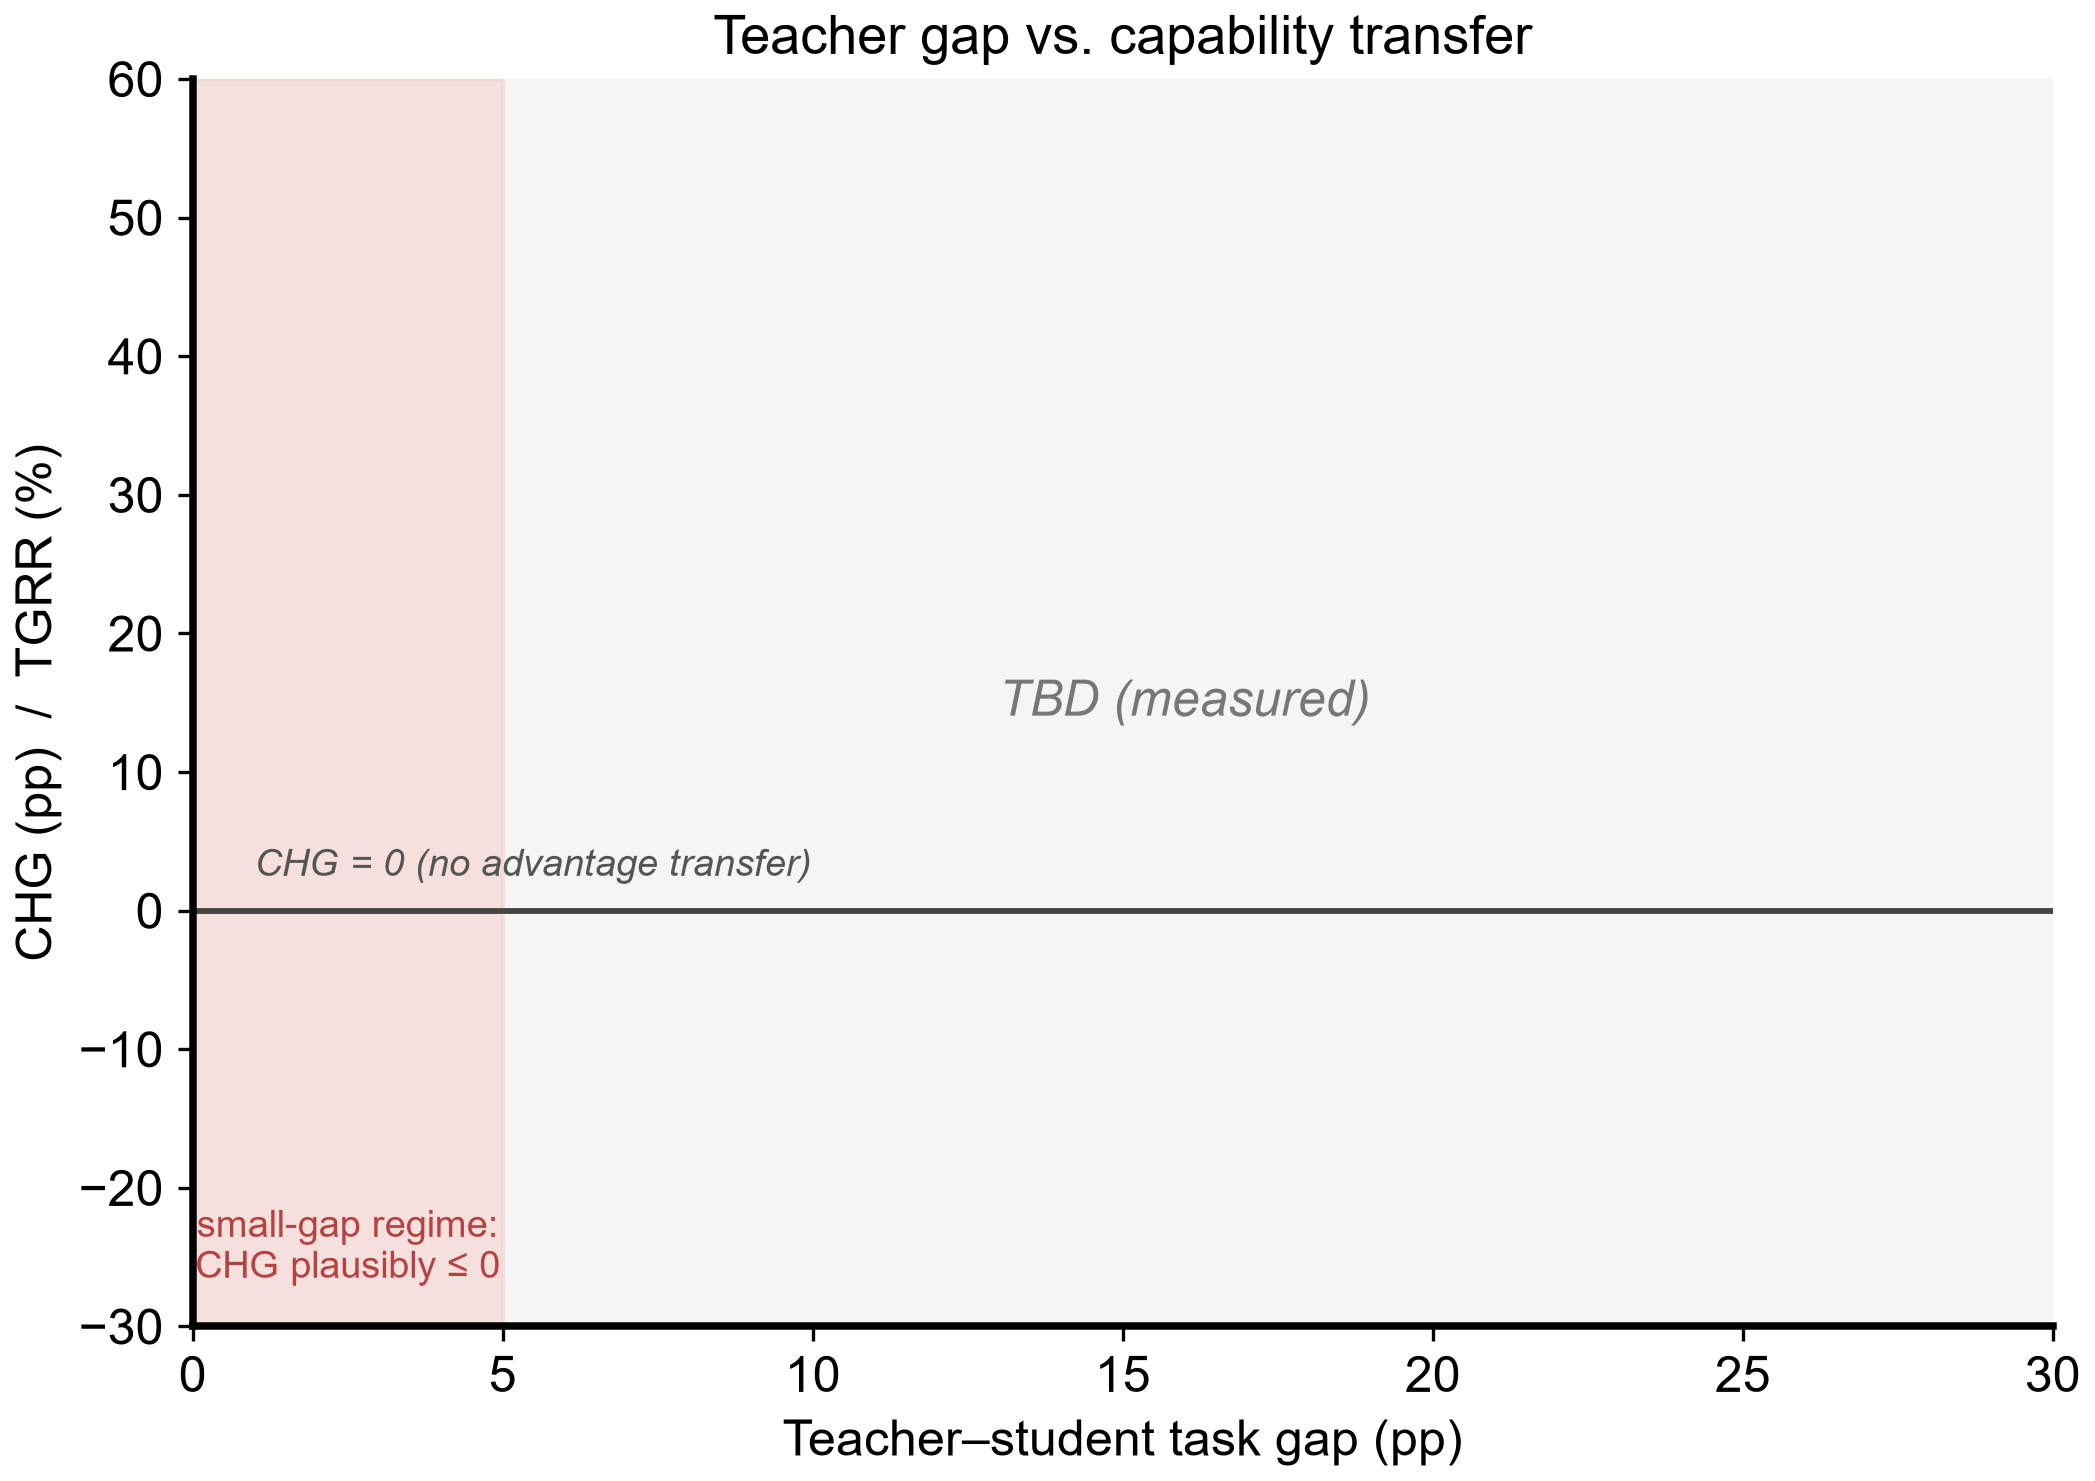
\includegraphics[width=0.62\textwidth]{figure4_teacher_gap.png}
\caption{Teacher gap versus \chg/\tgrr. The small-gap regime where \chg{} plausibly stays at or
below zero is marked; measured points are pending.}
\label{fig:gap}
\end{figure}

\subsection{Quality--Latency Pareto}
The projected Pareto landscape places ridge and the low-rank base in the ``prefill saving but
below self-prefill quality'' region with reasonable confidence, since both mappers are explicitly
optimized toward the student's own self-KV. \method{} is different: its plausible range straddles
$\chg=0$, so whether it actually enters the paper's target quadrant (positive \chg{} together
with positive \psr, roughly 8--16\% in the prior) is the open empirical question rather than a
foregone conclusion. This is therefore a decisive figure precisely because its outcome is
uncertain: if measured \method{} lands at $\chg\le0$, the manuscript should pivot to Efficient
State Handoff rather than continue to claim Runtime Capability Transfer; if it lands clearly above
zero and grows with teacher gap, that is the paper's central positive result.

\begin{figure}[t]
\centering
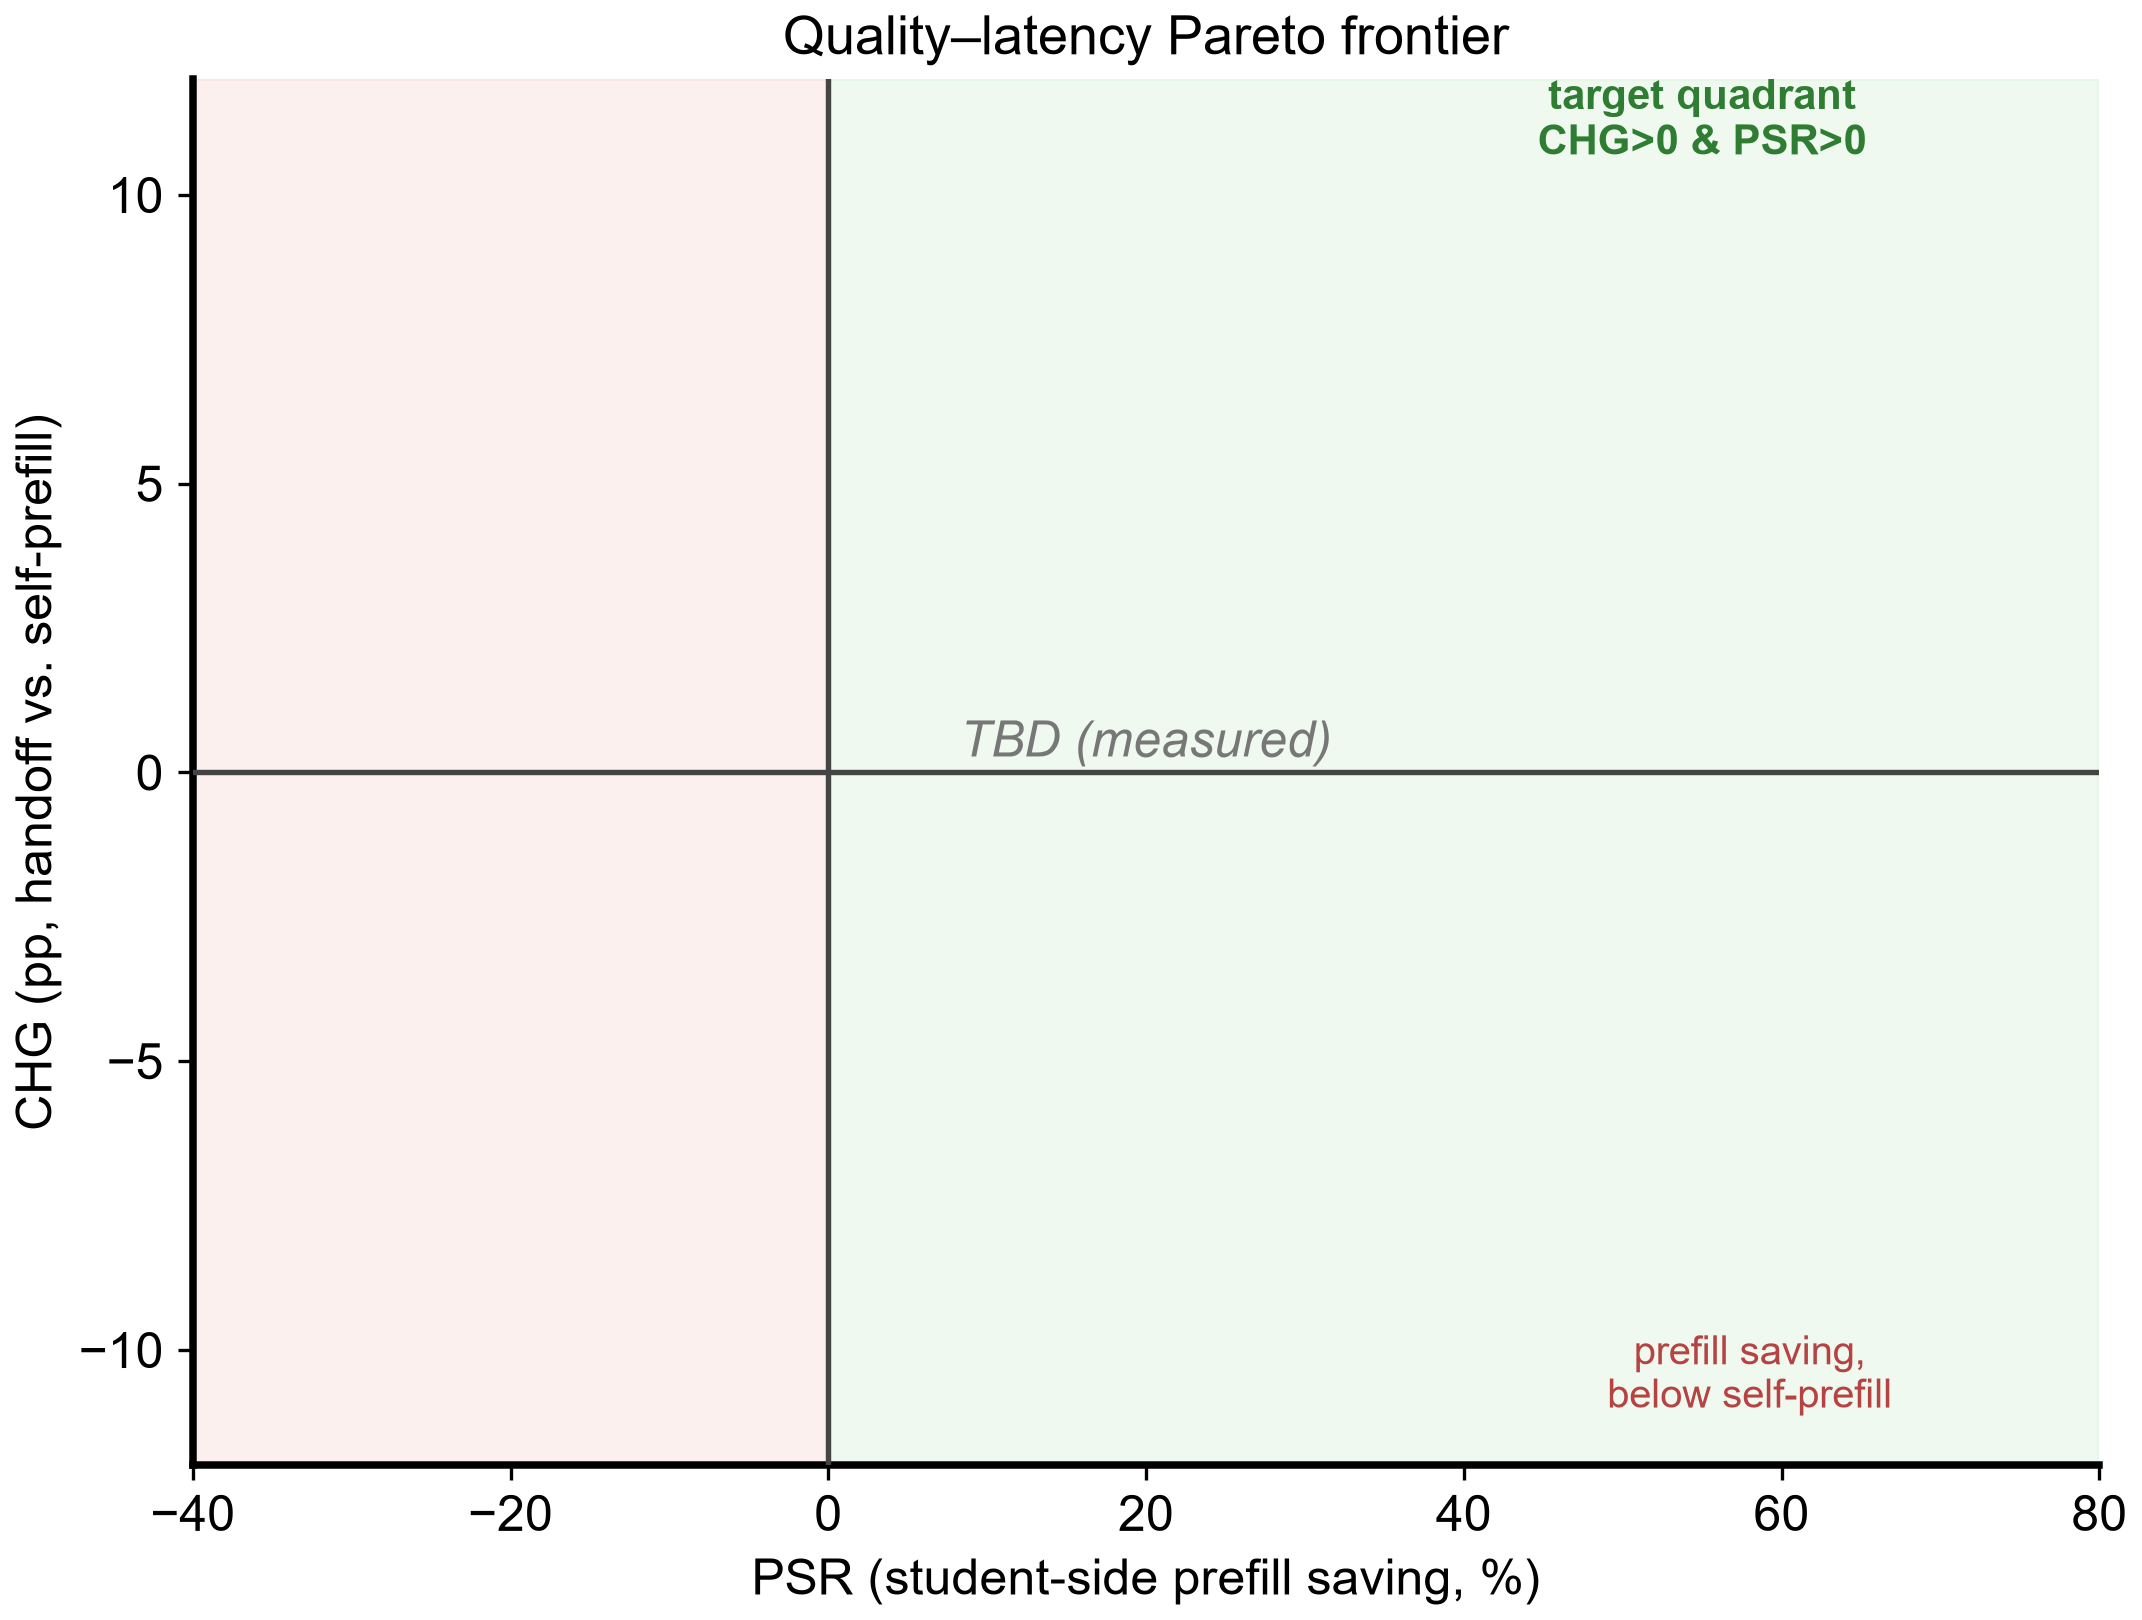
\includegraphics[width=0.64\textwidth]{figure5_pareto.png}
\caption{\chg/\tgrr--\psr{} Pareto frontier. The target quadrant ($\chg>0$ and $\psr>0$) is
marked; measured points are pending.}
\label{fig:pareto}
\end{figure}

\subsection{Context-Length Scaling}
The single-GPU cost prior predicts that map+load+query is slower than student full prefill at 1K
($\psr\approx-82\%$), and becomes progressively more favorable at longer contexts, but the exact
break-even point depends on an assumption we cannot yet verify: whether map/load overhead is
genuinely fixed or partly scales with context length. Under an optimistic fixed-overhead scenario
the crossover falls around 4K ($\psr\approx+12\%$) and reaches roughly $+48\%$ by 16K; under a
more conservative scenario where mapping cost itself grows with sequence length, the crossover
shifts out to somewhere between 4K and 8K and the 16K figure drops to roughly $+30\%$. We report
both scenarios rather than a single curve, and treat the true break-even as lying somewhere in
the 4K--8K range rather than a fixed point. This distinction matters because the pilot's
single-24GB-GPU setup requires sequential teacher/student residency (load $\rightarrow$ capture
$\rightarrow$ unload $\rightarrow$ load), which is a research-probe artifact rather than the
production regime that the map+load+query cost model describes; the measured study must separately
report model load/unload time, map time, cache H2D time, query-only prefill, and student
full-prefill latency so the two are not conflated.

\begin{figure}[t]
\centering
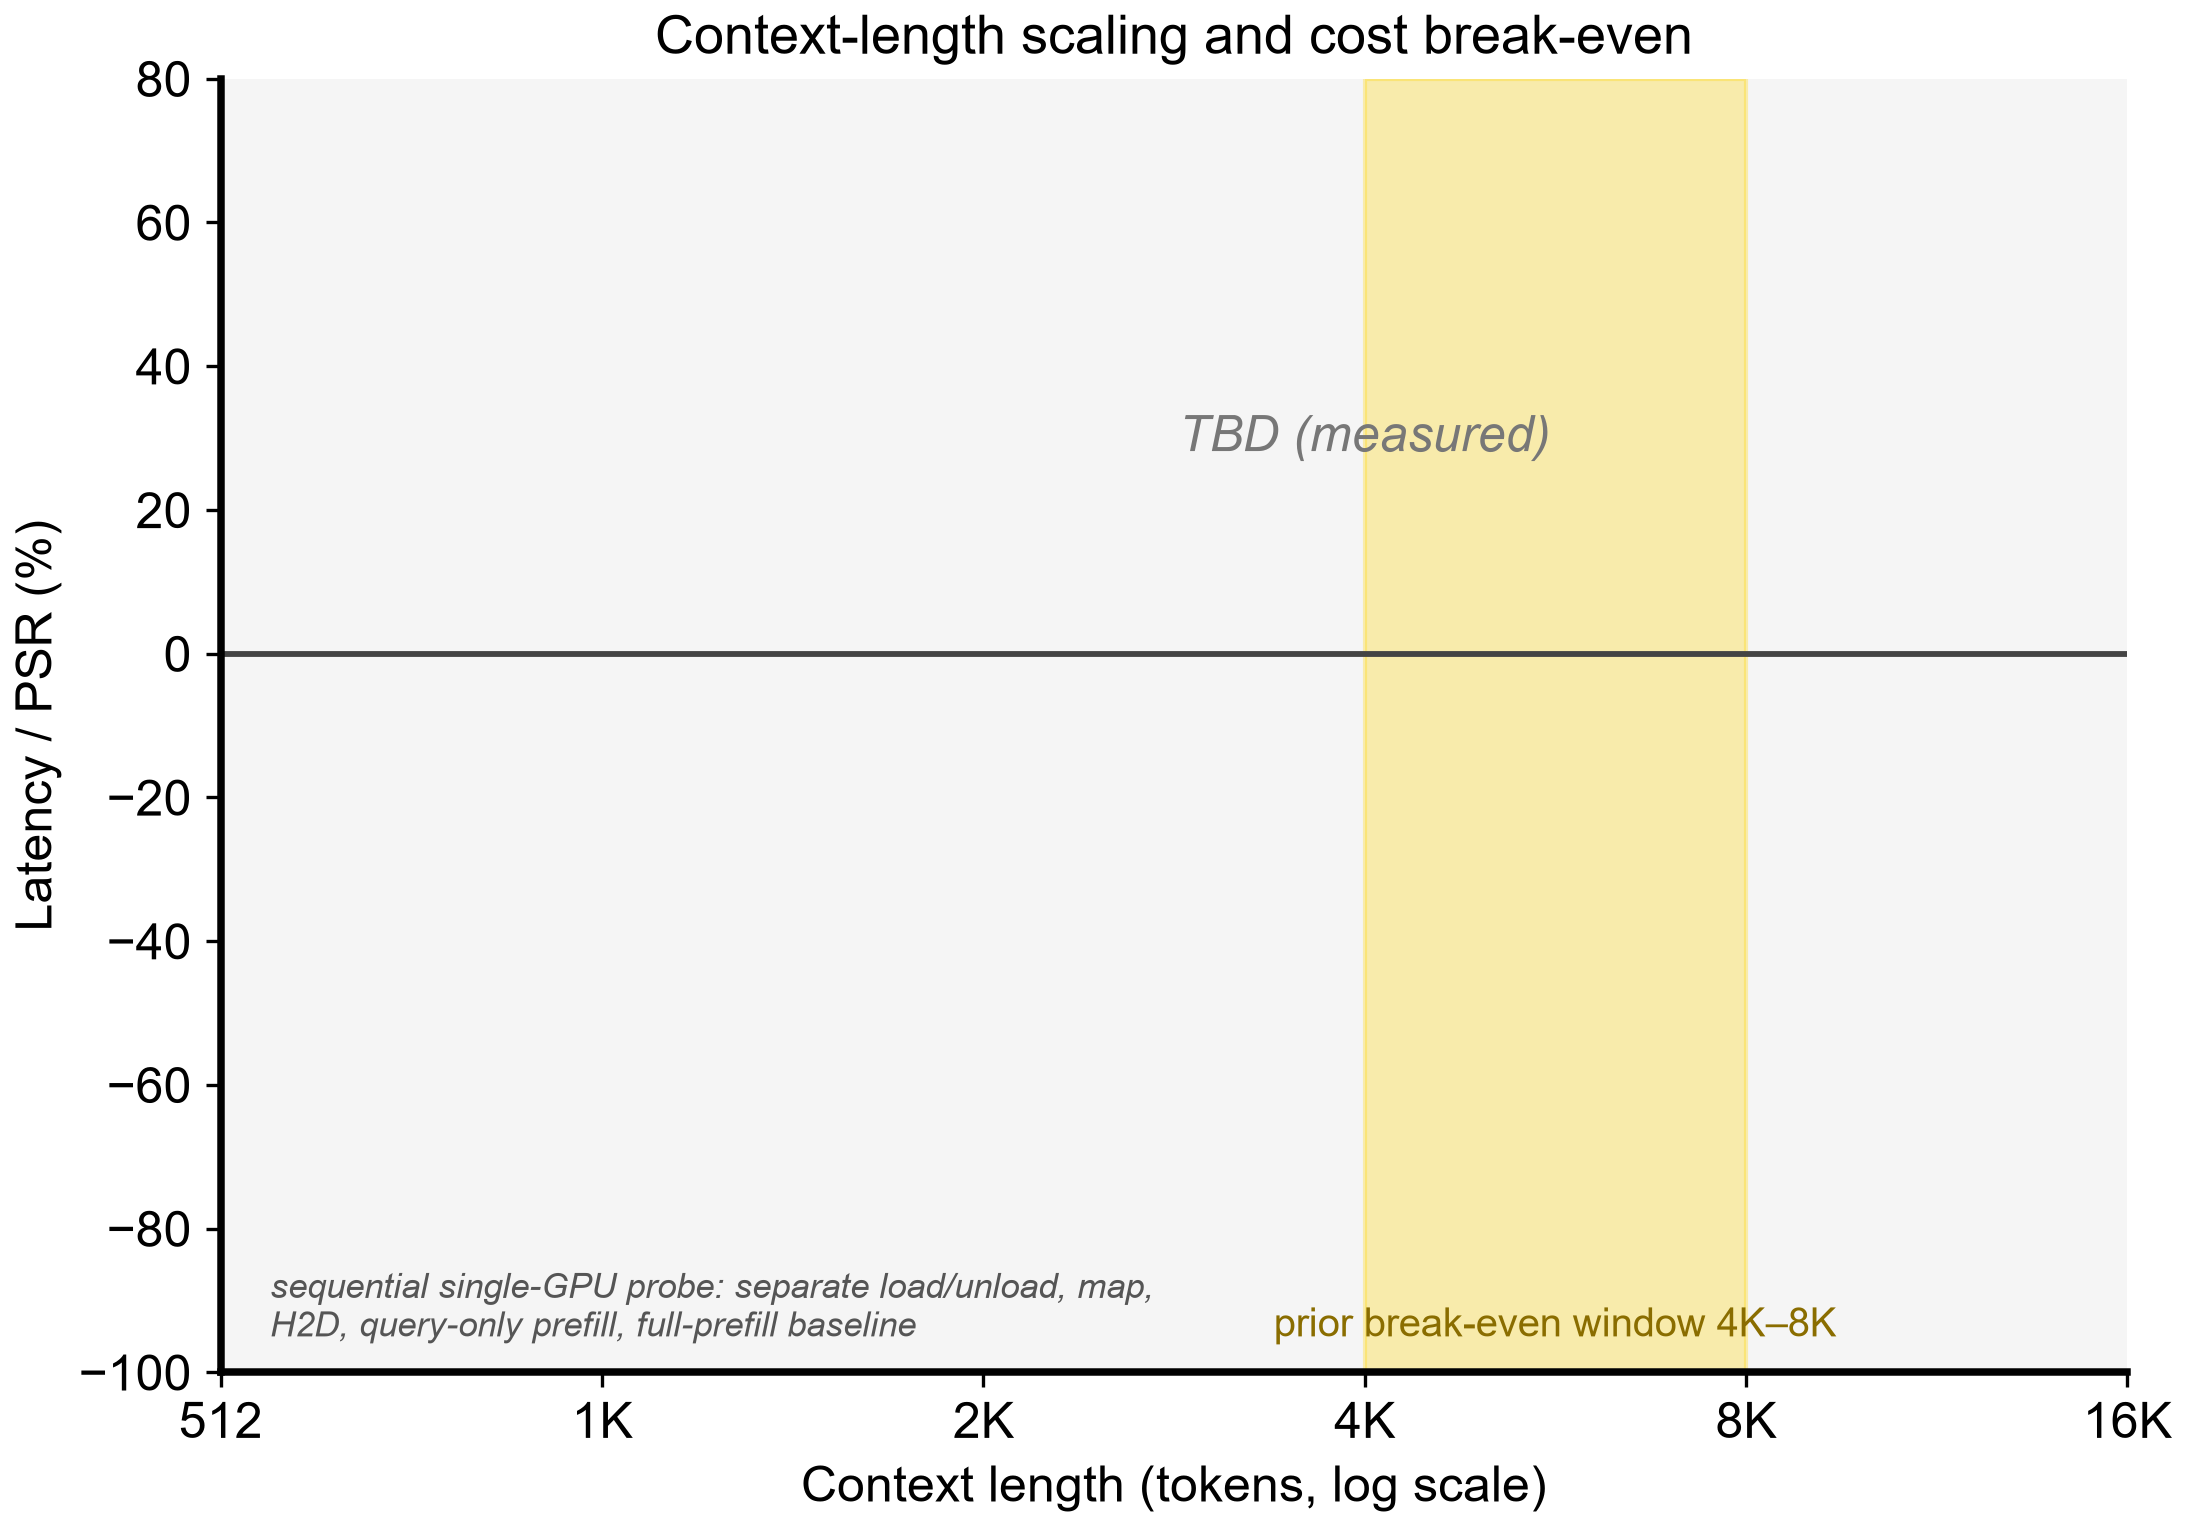
\includegraphics[width=0.62\textwidth]{figure6_context_length.png}
\caption{Context-length scaling and cost break-even. The 4K--8K window is a prior projection;
measured latency decompositions are pending.}
\label{fig:ctx}
\end{figure}

\subsection{Behavioral Stability and Multi-turn Handoff}
The multi-turn prior assumes gradual rather than catastrophic drift, but we now show it with a band
that widens over turns rather than a single smooth line, since uncertainty about drift compounds
the further we extrapolate from an untested turn-1 estimate: \chg{} plausibly falls from a range
of about 0.2--2.2 pp at turn 1 to a range of about $-2.1$--2.3 pp at turn 20, decision
consistency plausibly falls from roughly 97--98\% toward a range as wide as 84--90\% by turn 20,
and next-token KL rises with similarly growing uncertainty. The widening bands are the point: we
would not be surprised by a turn-20 \chg{} close to zero, and we do not treat the turn-1 central
estimate as a reliable predictor of long-horizon behavior. If measured drift is materially faster
than even the pessimistic edge of this band, periodic refresh or selective re-prefill should
become a primary follow-up rather than reporting only first-turn quality.

\begin{figure}[t]
\centering
\fbox{\parbox[c][3.2in][c]{0.62\textwidth}{\centering\itshape
Multi-turn behavioral stability (prior projection; measured points pending).}}
\caption{Multi-turn behavioral stability (prior projection; measured points pending).}
\label{fig:multiturn}
\end{figure}

\section{Planned Ablations}
The projected ablation hypothesis is that the compatibility base alone does not create positive
\chg; an advantage state is necessary for the capability signal; removing teacher guidance pushes
\chg{} back below zero; removing self-stability can increase short-term \chg{} at the cost of
larger behavioral drift; and directly mapping RoPE-encoded keys causes the largest retention
failure. Offline experiments should treat these as falsifiable predictions, not target numbers
that must be reproduced.

\begin{table}[t]
\centering
\caption{Core ablations, reported as plausible ranges. The Direct RoPE Mapping row uses a rounded
band rather than a suspiciously exact figure. The final analysis should distinguish mechanisms
that improve task-level handoff from those that only improve representation similarity.}
\label{tab:ablations}
\small
\begin{tabular}{lrrrrrl}
\toprule
Ablation & Retention & CHG & TGRR & PSR & PCR & Interpretation \\
\midrule
Full Ridge & 92--96\% & $-4.4$ to $-2.2$ & $-44$ to $-22\%$ & 3--8\% & 1.00 & High fidelity, expensive; no advantage transfer \\
Low-rank Base & 90--94\% & $-5.5$ to $-3.3$ & $-56$ to $-33\%$ & 12--20\% & 0.23 & Compact, but remains emulation \\
+ Advantage State & 98--104\% & $-1.0$ to $+2.0$ & $-10$ to $+20\%$ & 10--16\% & 0.27 & Initial positive capability signal \\
$-$ Teacher Guidance & 95--101\% & $-2.5$ to $+0.3$ & $-25$ to $+3\%$ & 10--16\% & 0.27 & CHG turns negative without teacher guidance \\
$-$ Self Stability & 100--106\% & $-0.2$ to $+3.2$ & $-2$ to $+32\%$ & 10--16\% & 0.27 & Higher CHG but projected behavioral drift \\
Direct RoPE Mapping & 79--90\% & $-11.5$ to $-5.5$ & $-115$ to $-55\%$ & 8--14\% & 0.27 & Position mismatch causes large fidelity loss \\
Full \method & 97--105\% & $-1.6$ to $+2.7$ & $-16$ to $+27\%$ & 8--16\% & 0.27 & Plausibly the best trade-off, but CHG range still includes zero \\
\bottomrule
\end{tabular}
\end{table}

\section{Discussion}
The experiments are designed so that their interpretation is fixed in advance. If \chg{} is
consistently positive, the analysis turns to where the advantage lives: whether \tgrr{} shows
reproducible structure across teacher gap, layer, head, task type, and context length. If \chg{}
stays at or below zero while replacement retention is high, the conclusion is that state
compatibility does not imply capability transfer.

\subsection{Negative Results and Direction Asymmetry}
Large-to-small transfer may be intrinsically more difficult than small-to-large transfer because
the student can have insufficient representational capacity or incompatible attention geometry for
teacher-specific state. If $\chg\le0$ while replacement retention remains high, an important
conclusion is that cross-model state compatibility does not imply capability transfer. If
capability transfer appears only for certain pairs, the representational geometry that predicts
directional success becomes a mechanism result in its own right.

\subsection{Systems and Security Boundaries}
\psr{} claims apply primarily when the teacher cache already exists because of an upstream task.
If the teacher is run solely to create transferable state, teacher prefill must be included and
the reuse break-even point reported. Persisted KV state may encode sensitive information about the
original context; productionization therefore requires cache lifecycle controls, access isolation,
encryption at rest/in transit, minimization of persisted state, and verifiable deletion.

\section{Conclusion}
The question we set out to test is whether a weaker student can skip full prefill of the original
context, consume only a stronger teacher's runtime state, and inherit part of the teacher's task
advantage. The present draft contains no measured answer; it fixes the probe, the expectations,
and the decision rule. The probe runs on a sub-12GB GPU, uses roughly 70 lines of code on top of
Transformers, and completes in under half a day (Sections~5.5 and Appendix~A). The final paper
claims Runtime Capability Transfer only if frozen-test experiments establish $\chg>0$ with a
confidence interval excluding zero, consistently positive \tgrr, and $\psr>0$. Otherwise it
reports Efficient State Handoff, or the boundary result that state compatibility does not imply
capability transfer.

\section*{Ethics, Security, and Reproducibility}
\textbf{Ethics and security.} The research does not require collection of personal data. If real
operational contexts are later used, data classification, de-identification, and KV-cache
lifecycle controls are required. We will report negative results, all seeds, and full frozen test
sets rather than selecting examples to manufacture positive \chg.

\textbf{Reproducibility.} The final artifact should pin model commits, tokenizer, dtype, attention
implementation, RoPE configuration, cache layout, random seeds, hardware, and context lengths.
Each run should preserve configuration, metrics, system measurements, and logs.

\textbf{AI use statement (update before submission).} Generative AI was used in preparing this
manuscript draft for structural planning, language drafting, and formatting. The authors remain
responsible for experimental decisions, code validation, data analysis, result interpretation,
reference verification, and all final scientific claims. This statement must be updated to match
actual usage and the ICLR policy in force at submission time.

\begin{thebibliography}{99}
\bibitem{vaswani2017attention} Vaswani, A., Shazeer, N., Parmar, N., et al. Attention Is All You Need. NeurIPS, 2017.
\bibitem{dao2022flashattention} Dao, T., Fu, D. Y., Ermon, S., Rudra, A., \& R\'e, C. FlashAttention: Fast and Memory-Efficient Exact Attention with IO-Awareness. NeurIPS, 2022.
\bibitem{dao2024flashattention2} Dao, T. FlashAttention-2: Faster Attention with Better Parallelism and Work Partitioning. ICLR, 2024.
\bibitem{kwon2023vllm} Kwon, W., Li, Z., Zhuang, S., et al. Efficient Memory Management for Large Language Model Serving with PagedAttention. SOSP, 2023.
\bibitem{qin2025mooncake} Qin, R., Li, Z., He, W., et al. Mooncake: Trading More Storage for Less Computation---A KVCache-Centric Architecture for Serving LLM Chatbot. FAST, 2025.
\bibitem{cheng2025lmcache} Cheng, Y., Liu, Y., Yao, J., et al. LMCache: An Efficient KV Cache Layer for Enterprise-Scale LLM Inference. arXiv:2510.09665, 2025.
\bibitem{heo2026crossmodel} Heo, T., Shafipour, R., Zhao, R., et al. Cross-Model KV Cache Transfer in LLM Families: A Closed-Form Linear Mapping for Prefill Reuse. arXiv:2608.03893, 2026.
\bibitem{fu2025c2c} Fu, T., Min, Z., Zhang, H., et al. Cache-to-Cache: Direct Semantic Communication Between Large Language Models. ICLR, 2026.
\bibitem{dery2026latentalign} Dery, L. M., Yahav, Z., Prior, H., Feng, Q., Shen, J., \& Szlam, A. Latent Space Communication via K-V Cache Alignment. arXiv:2601.06123, 2026.
\bibitem{rossi2026latentcacheflow} Rossi, M., Raghunath, P., \& Wu, E. Latent Cache Flow: Model-to-Model Communication Without Text. ICML, 2026.
\bibitem{liu2026droidspeak} Liu, Y., Huang, Y., Yao, J., et al. DroidSpeak: KV Cache Sharing Across Fine-tuned Model Variants. NSDI, 2026.
\bibitem{woo2026icarus} Woo, S., Kil, J., Kim, H., et al. ICaRus: Identical Cache Reuse for Efficient Multi-Model Inference. ICLR, 2026.
\bibitem{woo2026prefillshare} Woo, S., Kim, H., Shim, S., et al. PrefillShare: A Shared Prefill Module for KV Reuse in Multi-LLM Disaggregated Serving. arXiv:2602.12029, 2026.
\bibitem{kuzina2026kava} Kuzina, A., Pioro, M., \& Ehteshami Bejnordi, B. KaVa: Latent Reasoning via Compressed KV-Cache Distillation. ICLR, 2026.
\bibitem{liang2026kvjudge} Liang, S., Wang, Z., Chujiajia, Xia, P., Zang, H., \& Zhou, D. When KV Cache Reuse Fails in Multi-Agent Systems: Cross-Candidate Interaction is Crucial for LLM Judges. ACL, 2026.
\bibitem{yang2025qwen3} Yang, A., Li, A., Yang, B., et al. Qwen3 Technical Report. arXiv:2505.09388, 2025.
\bibitem{bai2023longbench} Bai, Y., Lv, X., Zhang, J., et al. LongBench: A Bilingual, Multitask Benchmark for Long Context Understanding. arXiv:2308.14508, 2023.
\bibitem{hsieh2024ruler} Hsieh, C.-P., Sun, S., Kriman, S., et al. RULER: What's the Real Context Size of Your Long-Context Language Models? arXiv:2404.06654, 2024.
\bibitem{chen2026longbenchpro} Chen, Z., Wu, X., Jia, J., et al. LongBench Pro: A More Realistic and Comprehensive Bilingual Long-Context Evaluation Benchmark. arXiv:2601.02872, 2026.
\end{thebibliography}

\appendix
\section{Reference Implementation and Engineering Details}
\subsection{Core Implementation: Ridge Fit and 4-Way Intervention}
All four interventions are operations on the HuggingFace \texttt{past\_key\_values} tuple. Step~1
extracts teacher and student KV on a 100-sample calibration set, de-RoPEs keys before fitting, and
computes per-layer, per-head ridge mappings $W_K$ and $W_V$ with the closed-form solution. Step~2
assembles the four KV combinations and evaluates perplexity on continuation tokens.

\textbf{1. Calibration capture and ridge fit.}
\begin{small}
\begin{verbatim}
# capture teacher KV (source state) and student KV (reference target)
def capture_kv(model, input_ids):
    out = model(input_ids, use_cache=True, output_hidden_states=False)
    return out.past_key_values          # tuple of (K, V) per layer

# de-RoPE keys before fitting; re-RoPE after mapping (Section A.2.1)
def derope_k(k, positions, inv=False):
    # k: [B, H, T, D] with D even; RoPE base shared by teacher and student
    D = k.shape[-1]
    theta = positions.float().unsqueeze(-1) / model.rope_base ** (
        torch.arange(0, D, 2, device=k.device).float() * 2 / D)
    cos, sin = theta.cos(), theta.sin()
    k1, k2 = k[..., 0::2], k[..., 1::2]
    if inv: k1, k2 = k2, k1             # inverse rotation (de-RoPE)
    return torch.cat([k1 * cos - k2 * sin, k1 * sin + k2 * cos], dim=-1)

def fit_ridge(Z, Y, lam=1e-3):          # per-layer, per-head [B,H,T,D]
    Zt = Z.transpose(-1, -2)
    return torch.linalg.solve(Zt @ Z + lam * torch.eye(D, device=Z.device), Zt @ Y)

# fit on the calibration set: W maps teacher KV to student KV
W_k, W_v = {}, {}
for l in range(student_layers):         # 28 student layers
    tl = int(round(l * (36 - 1) / (28 - 1)))     # layer alignment (A.2.2)
    W_k[l] = fit_ridge(Z_k_teacher[tl].flatten(0, 2), K_student[l].flatten(0, 2))
    W_v[l] = fit_ridge(Z_v_teacher[tl].flatten(0, 2), V_student[l].flatten(0, 2))
\end{verbatim}
\end{small}

\textbf{2. Four-way intervention PPL evaluation loop.}
\begin{small}
\begin{verbatim}
def evaluate_ppl(student_model, input_ids, custom_kv=None):
    with torch.no_grad():
        outputs = student_model(input_ids=input_ids, past_key_values=custom_kv,
                                labels=input_ids)
        return torch.exp(outputs.loss).item()

def mapped_kv(teacher_kv, W_k, W_v, positions):
    kv = []
    for l in range(student_layers):
        tl = int(round(l * 35 / 27))
        k = teacher_kv[tl][0]                      # teacher key, RoPE-encoded
        k = derope_k(k, positions, inv=True)       # de-RoPE content space
        k = k @ W_k[l]                             # ridge map to student
        k = derope_k(k, positions, inv=False)      # re-RoPE with student scheme
        kv.append((k, teacher_kv[tl][1] @ W_v[l])) # mapped K and V
    return tuple(kv)

# the 4 intervention arms switch only this tuple:
kv_case1 = (native_k, native_v)     # Native K + Native V (Baseline)
kv_case2 = (mapped_k, native_v)     # Mapped K + Native V
kv_case3 = (native_k, mapped_v)     # Native K + Mapped V
kv_case4 = (mapped_k, mapped_v)     # Mapped K + Mapped V (Full Handoff)
ppl = [evaluate_ppl(student, ids, kv)
       for kv in [kv_case1, kv_case2, kv_case3, kv_case4]]
\end{verbatim}
\end{small}

\textbf{Padding handling.} PPL is computed only on target (continuation) tokens; padding tokens
are excluded by setting their label to $-100$ (\texttt{ignore\_index}) rather than by removing
them from the sequence, so the attention and cache layout stays unchanged.

\subsection{Critical Engineering Details (Three Pitfalls)}
These details are not cosmetic. A nominal 512/1024-token experiment silently shrank to 70 tokens
in an earlier pipeline because of global cropping, and a value diagnostic accidentally used values
as both keys and values. The three rules below prevent that class of error.

\textbf{1. RoPE alignment.} Keys must be de-RoPE'd before ridge mapping and re-RoPE'd after
mapping (Eq.~\ref{eq:compat}); values are mapped in raw form. The teacher and student must share
the same RoPE base. Within Qwen3 the head dimension is 128 in both models, so the rotation can be
inverted channel-wise and no head re-indexing is required.

\textbf{2. Layer alignment (36 $\rightarrow$ 28).} We use a fixed 1-to-1 correspondence via uniform
linear interpolation, \texttt{teacher\_layer\_idx} $= \mathrm{round}(\texttt{student\_layer\_idx}
\times (36-1)/(28-1))$, and do not spend compute on learned layer-mixture weights in the first
version.

\textbf{3. Context-length bucketing and padding exclusion.} Test texts are strictly filtered or
truncated to $\texttt{max\_length} \in \{512, 1024, 2048\}$ before evaluation, and PPL must
exclude padding tokens from the loss (labels set to $-100$).

\section{Result Completion Checklist and Gated Workflow}
\begin{itemize}[leftmargin=*,nosep]
  \item Main table with at least two large-to-small pairs and full-test Student/Teacher/Ridge/\method{} results.
  \item Figure~\ref{fig:pcr}: PCR--Retention, establishing the mapper-budget/compatibility trade-off.
  \item Figure~\ref{fig:gap}: Teacher Gap--CHG/TGRR, supporting or falsifying runtime-advantage transfer.
  \item Figure~\ref{fig:pareto}: CHG/TGRR--PSR Pareto frontier as the primary paper figure.
  \item Figure~\ref{fig:ctx}: context-length scaling with absolute latency decomposition.
  \item Figure~\ref{fig:multiturn}: multi-turn behavioral stability with KL/JCR/consistency.
  \item Ablations on rank/shared basis, advantage state, teacher guidance, self stability, de-RoPE, and top-$k$ layers.
  \item The T00--T11 gated workflow: T00 Compatibility Scanner $\rightarrow$ T01 Self-KV Replay
  $\rightarrow$ T02 RoPE $\rightarrow$ T03 Layer Alignment $\rightarrow$ T04 Ridge $\rightarrow$
  T05 Replacement $\rightarrow$ T06 Lightweight Mapper $\rightarrow$ T07 Teacher Gap $\rightarrow$
  T08 Advantage State $\rightarrow$ T09 CHG/TGRR $\rightarrow$ T10 PSR $\rightarrow$ T11 MVP
  Decision. A failed gate blocks downstream claims so that every paper result is traceable to a
  verified engineering stage.
\end{itemize}

\end{document}
